%%%%%%%%%%%%%%%%
%% Preambule  %%
%%%%%%%%%%%%%%%%

\documentclass[11pt]{article}

\usepackage{amsmath,amsfonts,amssymb}
\usepackage{upgreek}
\usepackage{enumerate}
\usepackage{enumitem}   %
\usepackage{multicol}
\usepackage{scrextend}
\usepackage{fancyhdr}
\usepackage{lastpage}
\usepackage{subcaption} % 2 column images
\usepackage[all]{xy}
\usepackage{tikz-qtree}
\usepackage[margin=2.5cm]{geometry}


\setlength{\parindent}{0pt}

\pagestyle{fancy}

\lhead{\opdrachtNaam\ \opdrachtNummer}
\rhead{\naam(\studentNummer)}
\rfoot{Pagina\ \thepage\ van\ \pageref{LastPage}}
\lfoot{\datum}
\cfoot{}

\renewcommand\headrulewidth{0.4pt}
\renewcommand\footrulewidth{0.4pt}

\newcommand{\E}{\exists}
\newcommand{\A}{\forall}

\newcommand{\ccen}[2]{\llap{$#1$}${}\mathrel{\circ}{}$\rlap{$#2$}}

%%%%%%%%%%%%%%
%% Gegevens %%
%%%%%%%%%%%%%%

\newcommand{\naam}          {Stefan Schenk}
\newcommand{\studentNummer} {11881798}
\newcommand{\opdrachtNaam}  {Assignment}
\newcommand{\opdrachtNummer}{3}
\newcommand{\datum}         {November 2017}

%%%%%%%%%%%%%%%%
%% Antwoorden %%
%%%%%%%%%%%%%%%%

\begin{document}

% Opgaven:
%
% Opdrachten 4.2, 5.12, 5.23 van (1) tot (4), 5.26, 5.28,
% 5.49 (voor $ { \leftrightarrow, \neg } $ ), 5.52, \\
% Opdrachten 8 en 11 van het stuk “Inductiebewijzen”.

\subsection*{Opgave 4.2}

Als het niet waait dan is het half 3.

\underline{Het is half 3.\quad}

Het waait niet.


\subsection*{Opgave 5.12}

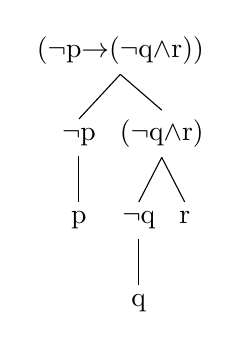
\begin{tikzpicture}
\Tree [.($\neg$p$\rightarrow$($\neg$q$\wedge$r)) [.$\neg$p [.p ] ]
  [.($\neg$q$\wedge$r) [.$\neg$q q ]
  [.r ]]]
\end{tikzpicture}

Het bereik van de negatietekens zijn respectievelijk p en de ander q.


\subsection*{Opgave 5.23}

\begin{enumerate}[label=(\arabic*)]

  % 1
  \item
  \begin{tabular}{c|c}
  $\varphi$ & $\varphi \vee \varphi$ \\
  \hline
  0 & 1 \\
  1 & 1 \\
  \end{tabular} \\

  Tautologie

  % 2
  \item
  \begin{tabular}{cc|c|c}
  $\varphi$ & $\psi$ & $(\varphi \wedge \psi)$
    & $(\varphi \wedge \psi) \rightarrow \varphi$ \\
  \hline
  0 & 0 & 0 & 1\\
  0 & 1 & 0 & 1\\
  1 & 0 & 0 & 1\\
  1 & 1 & 1 & 1\\
  \end{tabular} \\

  Tautologie

  % 3
  \item
  \begin{tabular}{cc|c|c}
  $\varphi$ & $\psi$ & $(\varphi \vee \psi)$
    & $\varphi \rightarrow (\varphi \vee \psi)$ \\
  \hline
  0 & 0 & 0 & 1\\
  0 & 1 & 1 & 1\\
  1 & 0 & 1 & 1\\
  1 & 1 & 1 & 1\\
  \end{tabular} \\

  Tautologie

  % 4
  \item
  \begin{tabular}{cc|cc|c}
  $\varphi$ & $\psi$ & $\neg \varphi$ & $(\varphi \rightarrow \psi)$
    & $\neg \varphi \rightarrow (\varphi \rightarrow \psi)$ \\
  \hline
  0 & 0 & 1 & 1 & 1\\
  0 & 1 & 1 & 1 & 1\\
  1 & 0 & 0 & 0 & 1\\
  1 & 1 & 0 & 1 & 1\\
  \end{tabular} \\

  Tautologie

  % 5
  \item
  \begin{tabular}{cc|c|c}
  $\varphi$ & $\psi$ & $(\varphi \rightarrow \psi)$
    & $((\varphi \rightarrow \psi) \rightarrow \varphi) \rightarrow \varphi$ \\
  \hline
  0 & 0 & 1 & 0\\
  0 & 1 & 1 & 0\\
  1 & 0 & 0 & 1\\
  1 & 1 & 1 & 1\\
  \end{tabular} \\

  Geen Tautologie

  % 6
  \item
  \begin{tabular}{ccc|ccc|c}
  $\varphi$ & $\psi$ & $\chi$ &
    $(\varphi \rightarrow \psi)$ &
    $(\varphi \rightarrow \chi)$ &
    $(\psi \rightarrow \chi)$ &
    $(\varphi \rightarrow (\psi \rightarrow \chi))
      \rightarrow
      ((\varphi \rightarrow \psi) \rightarrow (\varphi \rightarrow \chi))$ \\
  \hline
  0 & 0 & 0 & 1 & 1 & 1 & 1\\
  0 & 0 & 1 & 1 & 1 & 1 & 1\\
  0 & 1 & 0 & 1 & 1 & 0 & 1\\
  0 & 1 & 1 & 1 & 1 & 1 & 1\\
  1 & 0 & 0 & 0 & 0 & 1 & 1\\
  1 & 0 & 1 & 0 & 1 & 1 & 1\\
  1 & 1 & 0 & 1 & 0 & 0 & 1\\
  1 & 1 & 1 & 1 & 1 & 1 & 1\\
  \end{tabular} \\

  Tautologie

\end{enumerate}


\subsection*{Opgave 5.26}

$p\wedge q$

\subsection*{Opgave 5.28}

\begin{tabular}{cc|cc|c}
$\neg \varphi$ & $\neg \psi$ &
  $(\varphi \rightarrow \psi)$ \\
\hline
1 & 1 & 1 \\
1 & 0 & 1 \\
0 & 1 & 0 \\
0 & 0 & 1 \\
\end{tabular}
\\

De bovenste regel laat zien dat Modes Tollens geldig is.

\subsection*{Opgave 5.49}

Functioneel volledigheid: $\{\wedge, \neg\}$

\begin{tabular}{cc|c}
p & q & $\neg (p \wedge \neg q)$ \\
\hline
1 & 1 & 1 \\
0 & 1 & 1 \\
1 & 0 & 0 \\
0 & 0 & 0 \\
\end{tabular}
\\

Functioneel volledigheid: $\{\rightarrow, \neg\}$

\begin{tabular}{cc|c}
p & q & $(p \rightarrow p) \rightarrow q$ \\
\hline
1 & 1 & 1 \\
0 & 1 & 1 \\
1 & 0 & 0 \\
0 & 0 & 0 \\
\end{tabular}
\\

Functioneel volledigheid: $\{\vee, \neg\}$

\begin{tabular}{cc|c}
p & q & $\neg (p \vee \neg q) \vee q$ \\
\hline
1 & 1 & 1 \\
0 & 1 & 1 \\
1 & 0 & 0 \\
0 & 0 & 0 \\
\end{tabular}
\\

\subsection*{Opgave 5.52}

Connectieven $\{\wedge, \vee, \rightarrow, \leftrightarrow\}$ omschreven m.b.v.
$\dagger$. \\

\begin{tabular}{ccc|c|c|c|c}
p & q & $\dagger$
  & $(p \dagger p) \dagger (q \dagger q)$
  & $(p \dagger q) \dagger (p \dagger q)$
  & ?
  & ? \\
\hline
1 & 1 & 0  & 1 & 1  & 1 & 1 \\
0 & 1 & 0  & 0 & 1  & 1 & 0 \\
1 & 0 & 0  & 0 & 1  & 0 & 0 \\
0 & 0 & 1  & 0 & 0  & 1 & 1 \\
\end{tabular}
\\

\bigskip

Connectieven $\{\wedge, \vee, \rightarrow, \leftrightarrow\}$ omschreven m.b.v.
$\mid$. \\

\begin{tabular}{ccc|c|c|c|c}
p & q & $\mid$
  & $(p \mid q) \mid (p \mid q)$
  & $(p \mid p) \mid (q \mid q)$
  & ?
  & ? \\
\hline
1 & 1 & 0  & 1 & 1  & 1 & 1 \\
0 & 1 & 1  & 0 & 1  & 1 & 0 \\
1 & 0 & 1  & 0 & 1  & 0 & 0 \\
0 & 0 & 1  & 0 & 0  & 1 & 1 \\
\end{tabular}
\\

\subsection*{Inductiebewijzen 8}
Te bewijzen: iedere propositielogische formule waarin $\vee$ het enige
connectief is, waar is, iff tenminste een van zijn atomaire zinnen die in de
formule voorkomen waar is.

\textbf{Base case:} Er is geen connectief.

\textbf{I.H.:} Voor alle zinnen met minder compexiteit dan $\phi$ geldt de te
bewijzen stelling.

\textbf{I.S.:} - $\phi = \psi \vee \chi$. Volgens I.H. zijn $\psi$ en $\chi$
waar, dus $\psi$ is waar of $\chi$ is waar, dus $\phi$ is waar.
\hfill $\Box$

\subsection*{Inductiebewijzen 9}
Neem een taal zonder negatie en waarin geldt dat voor alle $p\in ATOM:V(p)=1$.
\smallskip

Te bewijzen: voor alle formules $\phi$ geldt dat $V(\phi)=1$.

\textbf{Base case:} $\phi$ = p, $V(p)=1$.

\textbf{IH:} Voor alle formules met minder compexiteit dan $\phi$ geldt de te
bewijzen stelling.

\textbf{I.S.:} \\
- $\phi = \psi \vee \chi:$ Volgens I.H. is $V(\psi)=1$, dus ook $V(\psi \vee
\chi)=1$.\\
- $\phi = \psi \wedge \chi:$ Volgens I.H. is $V(\psi)=1=V(\chi)$, dus ook $V
(\psi \wedge \chi)=1$.\\
- $\phi = \psi \rightarrow \chi:$ Volgens I.H. is $V(\chi)=1$, dus ook $V(\psi
\rightarrow \chi)=1$.
\hfill $\Box$


\pagebreak

\subsection*{Inductiebewijzen 10}
Te bewijzen: dat geldt voor alle formules uit de propositielogica, en alle
valuaties $V$, ofwel $V(\phi)=1$, ofwel $V(\phi)=0$, maar nooit $V(\phi)=1$ en
$V(\phi)=0$.

\textbf{Base case:} $\phi$ = p, $V(p)=1$ of $V(p)=0$, geldt voor een enkele
propositie.

\textbf{IH:} Voor alle formules met minder compexiteit dan $\phi$ geldt de te
bewijzen stelling.

\textbf{I.S.:} \\
- $\phi = \psi \vee \chi:$ Volgens I.H. is $V(\psi)=$ 1 of 0, dus ook $V(\psi
\vee \chi)$ = 1 of 0.\\
- $\phi = \psi \wedge \chi:$ Volgens I.H. is $V(\psi)=$ 1 of 0, net als $\chi$,
dus ook $V (\psi \wedge \chi)=$ 1 of 0.\\
- $\phi = \psi \rightarrow \chi:$ Volgens I.H. is $V(\chi)=$ 1 of 0, net als
$\chi$, dus ook $V(\psi \rightarrow \chi)$ = 1 of 0.
\hfill $\Box$


\subsection*{Inductiebewijzen 11}
Te bewijzen: dat elke formule waarin enkel de symbolen p,(,), $\rightarrow$ optreden een tautologie is of logisch equivalent is aan p.

\textbf{Base case:} $\phi$ = p, p zonder connectieven is gelijk aan p.

\textbf{IH:} Voor alle formules met minder compexiteit dan $\phi$ geldt de te
bewijzen stelling.

\textbf{I.S.:} \\
- $(\phi \rightarrow \phi) = \phi$ \\
- $(\phi) \rightarrow \phi = \phi$ \\
- $\phi \rightarrow (\phi) = \phi$
\hfill $\Box$

%%%%%%%%%%%%%%%%%%%%
%% Einde document %%
%%%%%%%%%%%%%%%%%%%%

\end{document}



